\documentclass[11pt,twocolumn]{article}
\usepackage{url}
\usepackage{breakurl}
\usepackage[breaklinks]{hyperref}
\usepackage{graphicx}
\usepackage{float}
\usepackage{appendix}
\begin{document}

\begin{titlepage} % Suppresses displaying the page number on the title page and the subsequent page counts as page 1
    \newcommand{\HRule}{\rule{\linewidth}{0.5mm}} % Defines a new command for horizontal lines, change thickness here
    
    \center % Centre everything on the page
    
    %------------------------------------------------
    %    Headings
    %------------------------------------------------
    
    \textsc{\LARGE Indiana University - Bloomington}\\[1.5cm] % Main heading such as the name of your university/college
    
    \textsc{\Large Network Science}\\[0.5cm] % Major heading such as course name
        
    %------------------------------------------------
    %    Title
    %------------------------------------------------
    
    \HRule\\[0.4cm]
    
    {\huge\bfseries Measuring Facebook Influence Using Centrality Measures and Community Detection}\\[0.4cm] % Title of your document
    
    \HRule\\[1.5cm]
    
    %------------------------------------------------
    %    Author(s)
    %------------------------------------------------
    
    \begin{minipage}{0.4\textwidth}
        \begin{flushleft}
            \large
            \textit{Authors}\\
            \textsc{Daniel Hinders\newline} % Your name
            \textsc{Nhi Tran} % Your name

        \end{flushleft}


    \end{minipage}
    ~
    \begin{minipage}{0.4\textwidth}
        \begin{flushright}
            \large
            \textit{Professor}\\
            \textsc{Yong-Yeol (YY) Ahn} % Supervisor's name
        \end{flushright}
    \end{minipage}
    
    % If you don't want a supervisor, uncomment the two lines below and comment the code above
    %{\large\textit{Author}}\\
    %John \textsc{Smith} % Your name
    
    %------------------------------------------------
    %    Date
    %------------------------------------------------
    
    \vfill\vfill\vfill % Position the date 3/4 down the remaining page
    
    {\large\today} % Date, change the \today to a set date if you want to be precise
    
    %------------------------------------------------
    %    Logo
    %------------------------------------------------
    
    %\vfill\vfill
    %\includegraphics[width=0.2\textwidth]{placeholder.jpg}\\[1cm] % Include a department/university logo - this will require the graphicx package
     
    %----------------------------------------------------------------------------------------
    
    \vfill % Push the date up 1/4 of the remaining page
    
\end{titlepage}

\title{Measuring Facebook Influence Using Centrality Measures and Community Detection}
\author{Daniel Hinders and Nhi Tran}
\maketitle
\begin{abstract}
Over the last few decades, social media has become a large part of life and society. With the aid of social media, social influence can be exerted by people, organizations, and government entities without physical human interaction. This project looks closely at the hallmarks of influential nodes and how to identify them in a social network. Additionally, the presence of communities and influential nodes in those communities was studied.  A public dataset of a subset of the Facebook social network sourced from November 2017 was used. Multiple network graph measurements and a community detection method were used to identify influential Facebook pages within a network. The analysis in this project identified several key nodes as highly influential in the network and their respective communities. The study also found that tools like Networkx and Gephi are excellent tools to formulate algorithmic-based evaluation to identify influence in a social network.\end{abstract}

\section{Introduction}

Social media amplifies individuals, organizations, and government agencies' ability to influence others.  This influence can be exerted anytime and even anonymously. It is important to be able to identify centers of influence within a social network. Without the tools to quickly identify influential nodes, a network can be too large to study and time-consuming for anyone to get useful information.    

\subsection{Background}

Social media impact has drastically increased its effect on life in the last 10-15 years, the diverse and far-reaching impacts cannot be overstated. Russian influence in the 2016 election, the Obama campaign utilizing social media to achieve a decisive victory in 2008, and social media fueling societal change and upheaval in the middle east and Hong Kong are some of the examples. 

In another realm, corporations spend a massive 11.6 percent \cite{social-media-pricing} average of their marketing through social media indicating a vast impact on society's choices and buying habits through social media.  

Amid these large organizations and vast movements in social media, there is a fascinating and powerful impact propagated through lone individuals on social media.  A single individual operating as a social media influencer is an existence that has become increasingly common in our societal vernacular. For many, a full-time job as a social influencer has become a viable career. 

Understanding all of these social media forces and impacts is important on many levels. Devastating negative ramifications: a nation-state subverting democracy by impacting other countries’ elections, hate groups spreading and inciting violence, and webs of misinformation leading to widespread distrust are all reasons alone to understand social media impact and influence. 

\subsection{Motivation and Objectives}

This project's goal is to analyze a public Facebook Page-to-Page network to identify important nodes and important nodes within different communities. In addition, this project seeks to identify methods, tools, and algorithms to evaluate influence in a social network. 

To achieve this goal, an objective was established to observe the differences between multiple centrality measurements and ultimately identify influential nodes within a network. The objective is pursued evaluating if degree centrality(the number of connections a node has with other nodes in the network) is sufficient to definitively identify influential nodes in a network.


A second objective was established to further pursue the project’s goal. The objective was to evaluate communities that exist around important nodes and also to determine if types of nodes in the network, in this network four different node page types, will be the basis around which communities in the network are formed.


\subsection{Existing Work}

Social media is increasingly prevalent in commerce, politics, and all societal interaction. Unsurprising, research seeking to measure and understand social media influence and impact is prevalent. 

Several studies are related to our project objectives. Some of them use similar centrality measures and some community detection techniques. 

\paragraph{A Comparative Study of Modularity-Based Community Detection Methods for Online Social Networks \cite{modularity-based-community}}   
 
In this paper, Karatas and Sahin focus on finding communities in social networks using modularity. The study assesses datasets from multiple social media platforms using different static community detection algorithms and specifically focuses on "modularity values, running time and accuracy"\cite{modularity-based-community} and compare and contrast these different algorithms for community detection assessing their strengths and weaknesses. The performance of the different algorithms was analyzed by measuring their modularity value, F1-score, and running time. Five different algorithms were used and the Louvain algorithm performed the best overall. The study suggests the following as problems with the currently available community detection algorithms: stability, scalability, refinement on computational complexity, dynamicity, and prediction. These ideas prompt and encourage future research on community network structure and the development of new community detection algorithms.

\paragraph{Social Circles in Facebook communities \cite{social-network-networkx}}   

The Social Circles in Facebook Communities study used the egonet dataset to assess specific subsets of the Facebook network which they termed social circles. Social circles are smaller groups within an individual's social network such as friends from high school or the workplace. The study utilized the egonet data set to construct various models of social circles and calculate Min Edit Distance and was purposed to: "predict what communities would form or what circles can be created using the given friendships" \cite{social-network-networkx}. Initially Clique Percolation to model the social circle data, but later in the study, the researchers found that Spectral Clustering was more effective. "Spectral Clustering is a way to cluster based on 'Affinity' and connectivity" \cite{social-network-networkx}. Our paper perhaps is a logical partner and expansion of this study. In the future perhaps integrating these two concepts would beneficial. The incorporation influence assessment might be a beneficial step towards identifying how communities would form around influential nodes.


\paragraph{Social Network Analysis with NetworkX \cite{social-network-networkx}}

This study used the Python library NetworkX to analyze network data from Facebook in graphic form. Using the Facebook ego network which structures data along a central vertex, the exercise started by analyzing betweenness centrality to determine the most connected individuals present in the dataset. After calculating betweenness centrality, the highest scoring 10 in the dataset were placed as central hubs within the graph. The next different communities were identified using community detection algorithms focusing on the modularity of the network or the fraction of edges. 

\paragraph{Network Analysis of Page Likes from Facebook User Profiles \cite{page-likes-facebook}}

This study is unique because instead of analyzing social media network data where the nodes represent individuals connected to other individuals, they place Facebook pages representing companies instead of individuals as the nodes and connect them to people based upon page likes. Using the myPersonality application, Facebook pages with at least 100 likes were included as nodes, and data were analyzed by calculation of clustering coefficient, diameter, and average path length. The study found that “the network’s in-degree distribution follows a power law” \cite{page-likes-facebook}. The study concludes that the structure of social media networks is consistent with small-world networks which are “characterized by dense local clustering and a short average path length between pairs of nodes” \cite{page-likes-facebook}. Our project incorporates some of the methods and objectives of this study and helped shape the project goals.

\section{Process and Approaches}

\begin{figure}[hbt!]
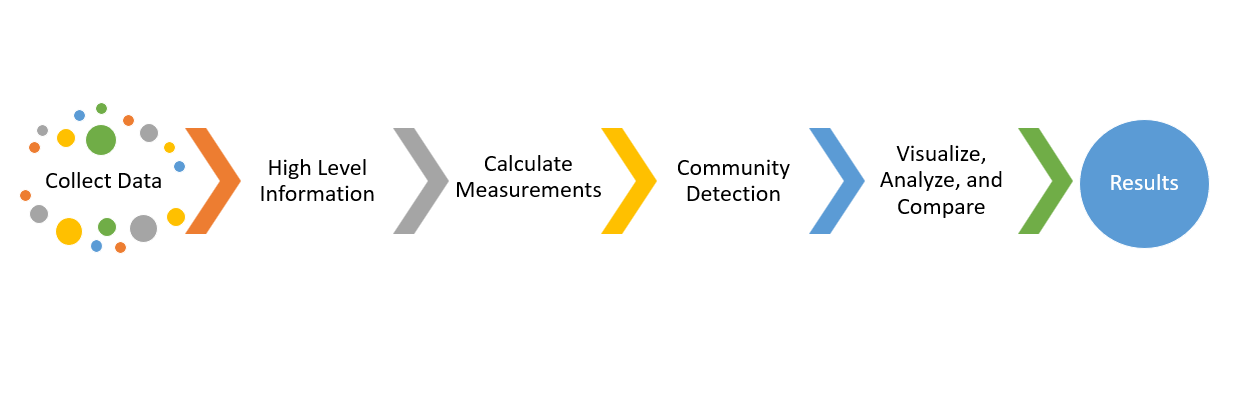
\includegraphics[scale=0.2]{process_flow.PNG} 
\caption{High Level Process}
\end{figure}

\textbf{Figure 1} identifies the steps that are necessary to complete the objectives of this report. Data was collected from the Stanford Network Analysis Project. Once the data are collected, the next would be to clean up the network graph, perform high-level analysis, calculations, detection community method. Then, all findings will be analyzed, visualized, and compared to get final results.

\subsection{Collecting Data}

\paragraph{Dataset \cite{page-page-network-ds}}
The dataset is November 2017 Facebook Large Page-Page Network from Stanford Network Analysis Project \cite{page-page-network-ds}. The dataset is a compressed zip file that contains the following files :
\begin{itemize}
\item\textbf{\texttt{musae\_facebook\_edges.csv}} – File that contains all edges between pages
\item\textbf{\texttt{musae\_facebook\_features.json}} – JSON file that contains features of the nodes - this file will not be used.
\item\textbf{\texttt{musae\_facebook\_target.csv}} - File that contains list of node ids, page names, and page types.
\end{itemize}

Each edge represents a mutual like between pages and each node is a Facebook page. There are four categories classifies for the Facebook pages: governmental organizations, politicians, television shows, and companies. The raw data contains 22,470 nodes and 171,002 edges.

\subsection{Data Cleaning and High-Level Information}

\paragraph{Tools}
The following software and tools were used to perform the analysis:
\begin{itemize}
\item \textbf{Python and Python Packages} - Python packages include Networkx, Pandas, and Matplotlib
\item \textbf{Jupyter Notebook}
\item \textbf{Gephi} - visualization and analysis tool for network graph
\end{itemize}

\paragraph{Cleanup}
After using Pandas Python package to read and combine the edges list and pages categories information csv files, the next step would be converting the data into graph object and removing self-loops, edges that connect a node to itself. After removing self-loops, the total edge count reduced from 171,002 to 170,823.

\paragraph{High-Level Information} 
The average degree is 15.2045, which means that on average, each node connects to about 15 other nodes. 

\begin{figure}[hbt!]
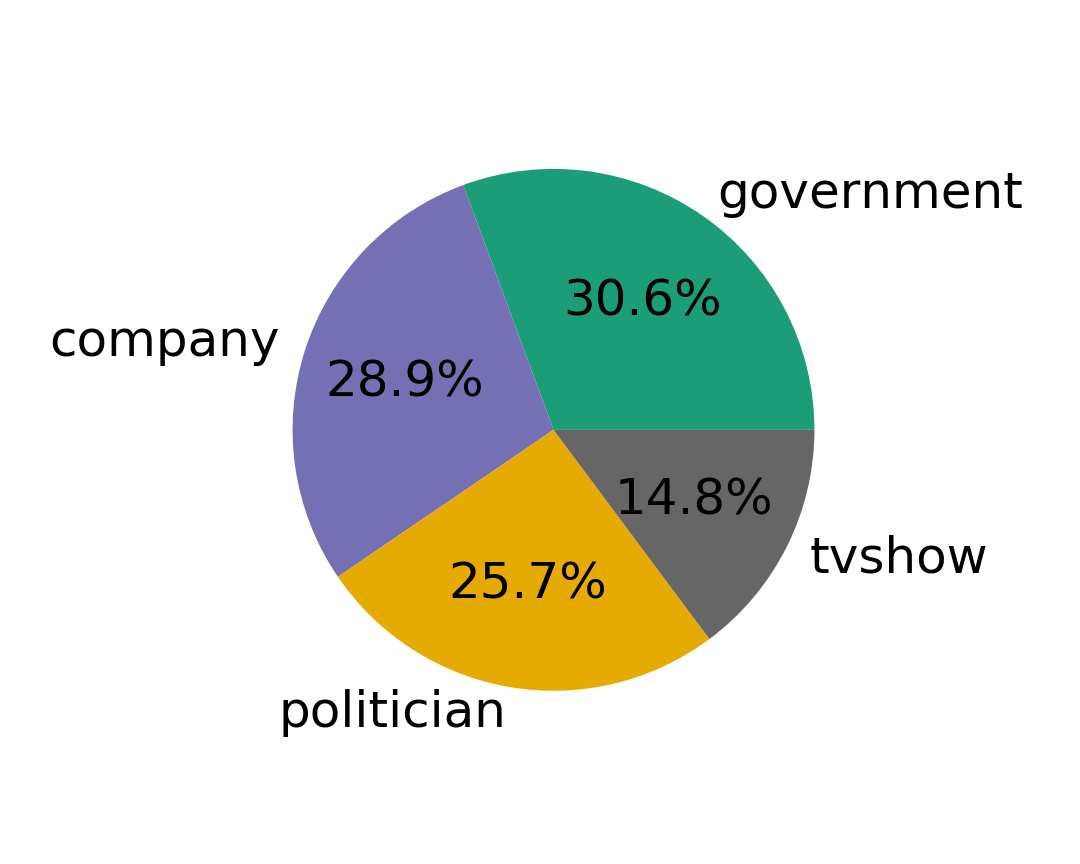
\includegraphics[scale=0.2]{pie_chart_category.png} 
\caption{Percentage of Page Category}
\end{figure}

\textbf{Figure 2} provides the composition of page categories within the network.


\begin{figure}[hbt!]
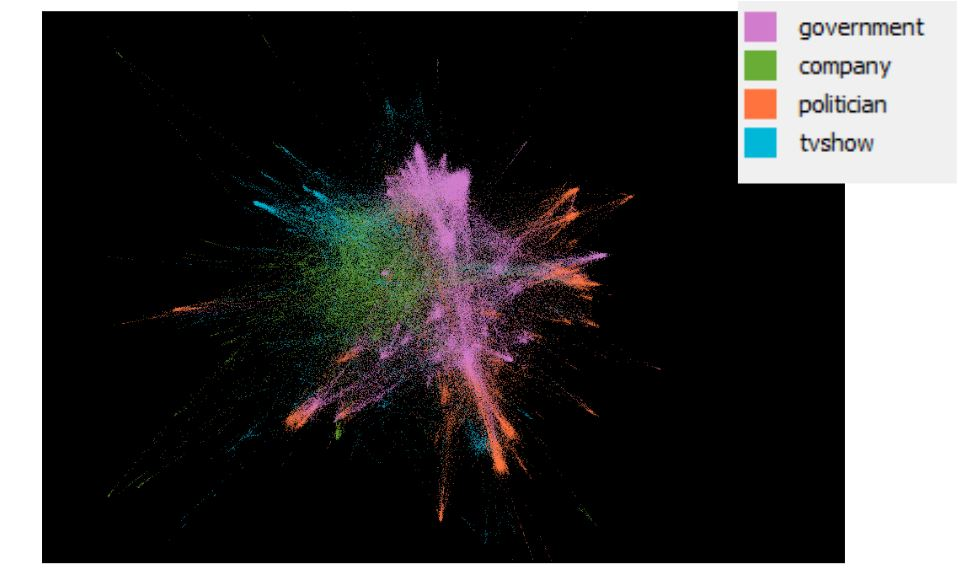
\includegraphics[scale=0.35]{gephi_whole_network_composition.JPG} 
\caption{Whole Network Visualization by Page Category}
\end{figure}


The same composition can be shown and visualized using Gephi as shown in \textbf{Figure 3}. One advantage of using Gephi over the pie chart is the visual of clustered areas within a network. There are a highly connected area and some small clustered areas within governmental organization pages. Politicians and tv show pages also have more clustered areas toward the outer part of the graph and Company pages don't have any obvious cluster. 

However, graphing the whole population makes it difficult to get more information out of the network. One way to work around that is to filter the network into a smaller network of high degree nodes for more observations. By filtering the whole network to only select giant components with higher-than-100-degree nodes, it resulted in a smaller network that only contains 314 nodes with 5,686 edges.


\begin{figure}[hbt!]
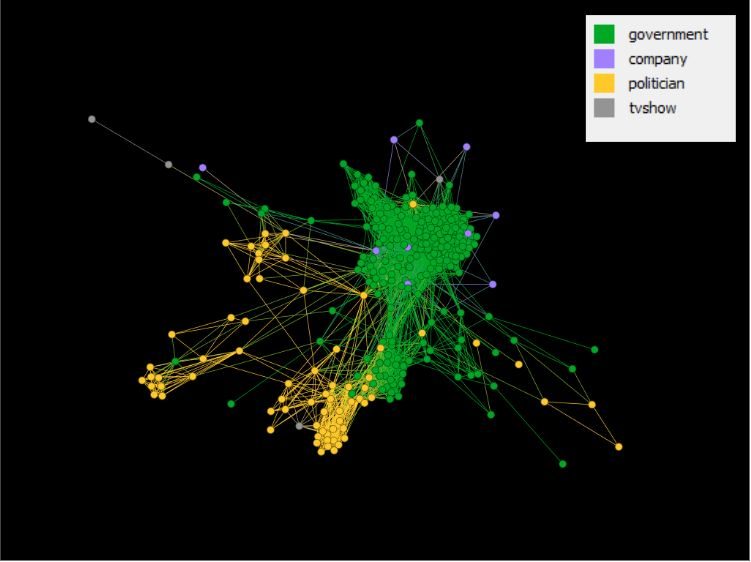
\includegraphics[scale=0.4]{gephi_filtered_100_degree.JPG} 
\caption{Visualization of Network with Nodes Greater Than 100 Degree}
\end{figure}

\textbf{Figure 4} shows that governmental organizations and politicians pages made of the majority of the population in a network of higher-than-100-degree nodes. It is also quite easy to identify the cluster areas (about 5 areas).

Another high-level measurement that is important and perhaps the most obvious measure of influence was a measurement of the degree of every node in the network. Degree centrality provides a simple yet telling quantitative data point for the number of edges or connections a given node has \cite{newman2008mathematics}.

\begin{figure}[hbt!]
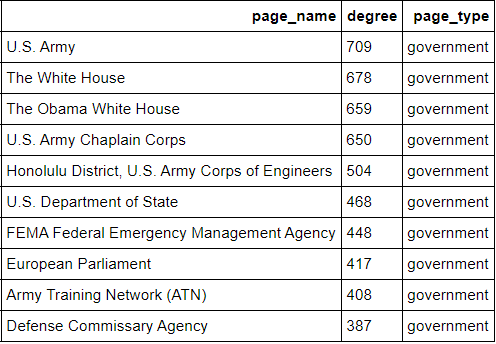
\includegraphics[scale=0.5]{top_ten_degree.png} 
\caption{Top Ten Highest Degree Pages}
\end{figure}

\textbf{Figure 5} contains the list of the top ten nodes that have the highest degree centrality within the whole network. One observation is that all of them are governmental organization pages; it aligns with the high composition of governmental organization pages shown in \textbf{Figure 4} earlier. It is interesting to see that the top five highest nodes are the United State's related pages. Is it because the majority of Facebook users are in the United States or were the data skewed? Those are the questions that should be answered before making business or important decisions using this dataset.

\begin{figure}[hbt!]
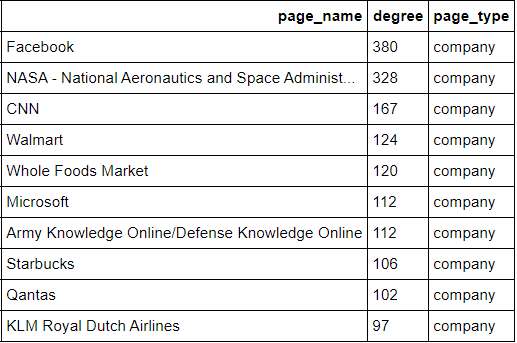
\includegraphics[scale=0.4]{top_ten_degree_company.png} 
\caption{Top Ten Highest Degree Company Pages}
\end{figure}
\begin{figure}[hbt!]
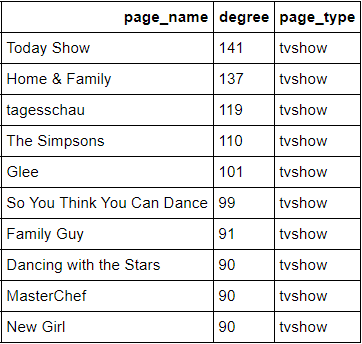
\includegraphics[scale=0.57]{top_ten_degree_tvshow.png} 
\caption{Top Ten Highest Degree TV Show Pages}
\end{figure}

\begin{figure}[hbt!]
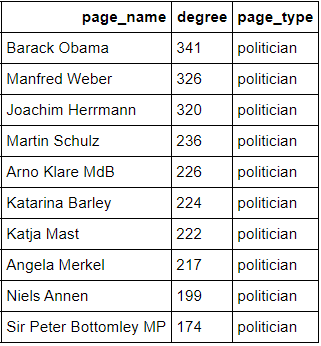
\includegraphics[scale=0.7]{top_ten_degree_politician.png} 
\caption{Top Ten Highest Degree Politician Pages}
\end{figure}


An additional filter of page type was added to get the top ten highest nodes of company pages, television shows, and politicians shown in \textbf{Figure 6}, \textbf{Figure 7}, and \textbf{Figure 8} respectively.  

Both of the top highest nodes under company and politician pages are about half of the degree amount comparing to the highest node in governmental organization pages. Television show pages seem to have the least influential power within this network.

\subsection{Calculate Measurements }
Other centrality measurements can be used to identify influential nodes within a network. It is important to understand the similarities and differences between these measurements and degree centrality to help with future network analysis. If degree centrality yields similar results to the rest of the other measurements, it might save time for researchers and scientists from having to calculate and perform deep-dive analysis.

\subsubsection{Betweenness Centrality} 
One of the useful centrality measurements to analyze a network is betweenness centrality. Betweenness centrality finds the path between every node in the network, then finds the shortest path and the nodes that fall into most of these shortest paths will have the highest betweenness score \cite{newman2008mathematics}. 

\begin{figure}[hbt!]
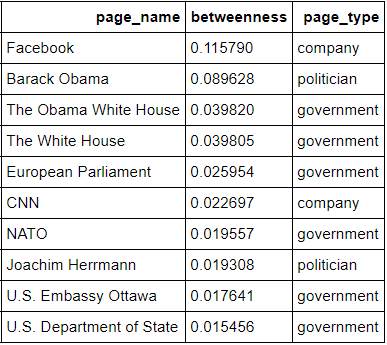
\includegraphics[scale=0.5]{top_ten_betweennness.png} 
\caption{Top Ten Highest Betweenness Centrality}
\end{figure}

\textbf{Figure 9} contains the top ten highest betweenness centrality nodes. The top ten nodes as calculated by their betweenness scores provides six governmental organization nodes, two politicians, and two companies. The range of the scores is between 0.0155 for the 10th highest and 0.116 for the 1st highest score.


\subsubsection{Closeness Centrality}
The next centrality measurement to analyze is closeness centrality. Closeness centrality provides the average path length between one node to every other vertex \cite{newman2008mathematics}.

\begin{figure}[hbt!]
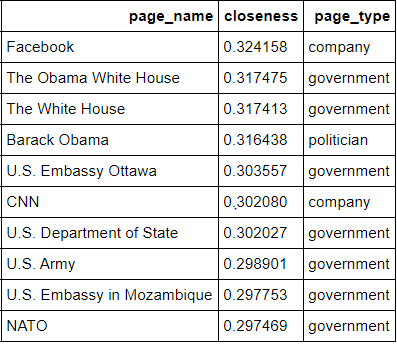
\includegraphics[scale=0.5]{top_ten_closeness.png} 
\caption{Top Ten Highest Closeness Centrality}
\end{figure}

\textbf{Figure 10} provided two companies, one politician, and seven governmental organizations in the top ten overall nodes with the highest Closeness centrality scores. The 10th highest had 0.0297 and the highest had 0.324.


\subsubsection{Eigenvector Centrality} 

Lastly, Eigenvector centrality needs to be measured for this network. Eigenvector centrality measures the connections a node has, not just the quantity, but also the quality or the influence of those connected nodes. A high Eigenvector score would indicate that a node is connected to many other highly influential, high scoring nodes \cite{newman2008mathematics}. 
 
\begin{figure}[hbt!]
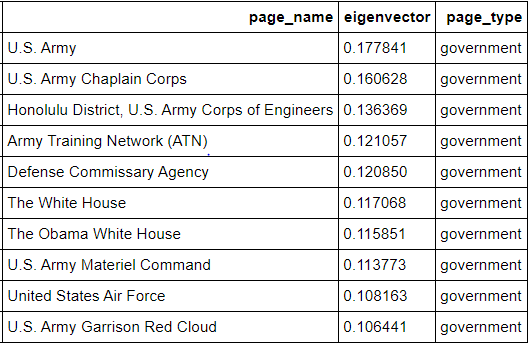
\includegraphics[scale=0.4]{top_ten_eigenvector.png} 
\caption{Top Ten Highest Eigenvector Centrality}
\end{figure}

Similar to degree centrality, the top ten Eigenvector nodes are government-related page types.  The range of the top ten eigenvector nodes ranges from 0.106 to 0.178 shown in \textbf{Figure 11}.

\subsection{Community Detection - Modularity}
The second objective evolves around the idea of community within a network and method to detect those communities. According to a research article called "Defining and Identifying Communities in Networks", a community is a group of nodes that have more dense connections between themselves comparing to the rest of the network \cite{Radicchi2658}. One of the popular methods to detect community is by using Modularity measurement. Modularity is "the portion of the edge connections within the same cluster minus the expected portion if the connections were distributed randomly" \cite{li_modular}.

Gephi can calculate and divide a network into each Modularity Class by providing a resolution number. According to Gephi's instruction, the higher the resolution value, the fewer the modularity classes there are. By providing a resolution value of 10, Gephi detected 8 modularity classes. Half of the modularity classes made up 98.37\% of the entire population; therefore, they can be the main four communities to compare to the four categories of Facebook pages (see \textbf{Figure 12}). 

\begin{figure}[hbt!]
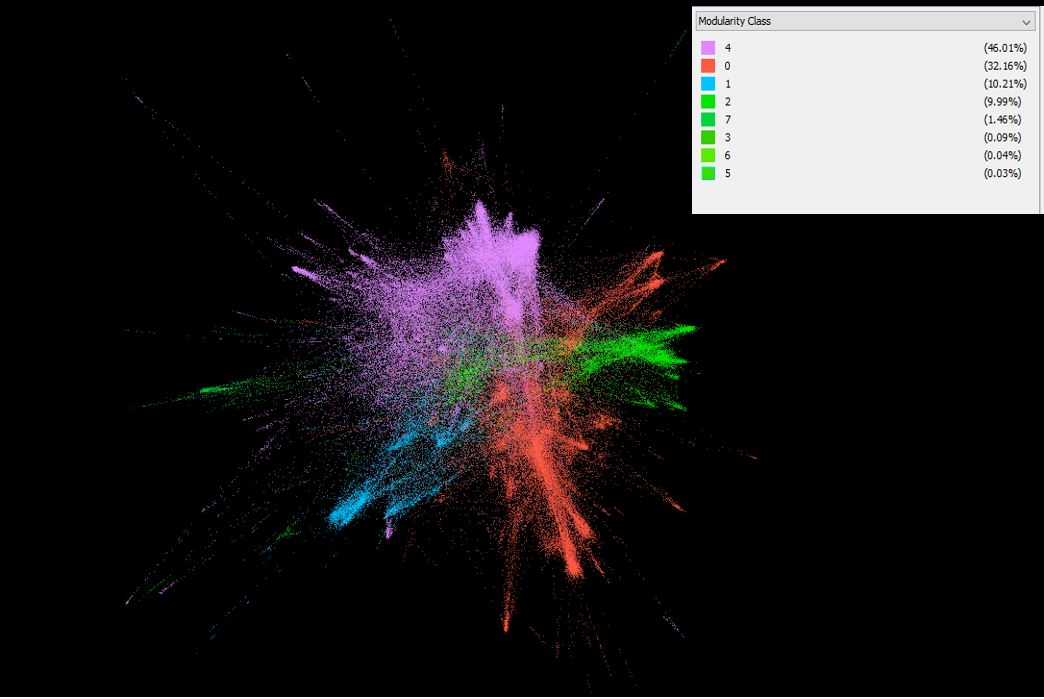
\includegraphics[scale=0.28]{modularity_community.JPG} 
\caption{Modularity Classes Graph}
\end{figure}



\section{Visualize, Analyze and Compare}

\subsection{Analysis and Comparison Methods}
Network Science provides concepts and approaches to help measure influence from analysis, foremost of these approaches is an algorithmic tool to evaluate nodes, edges, communities in a network. Using these tools, the objective measurement was possible to evaluate the importance and influence in a network like the Facebook dataset that was selected for this study. The selection of the algorithms used to measure influence was done carefully to address the measure influence from as many objective angles as possible. The analysis was conducted to measure centrality, community structure, and overall importance of nodes in the Facebook dataset.

\subsection{Comparing Degree Centrality to other Centrality Measurements}

\subsection{Visualizing and Analyzing Network of Each Page Category}
One area that needs more exploration is identifying influential nodes per each page category. When exploring the entire network as a whole, government pages were the majority of the resulted influential nodes. However, in some cases, there might be a specific need to know the influential nodes of each category. Therefore, instead of exploring the entire network as a whole, it is beneficial to filter the network by page type to analyze the network of each page category using betweenness, closeness, and Eigenvector centrality measurements. 

\subsubsection{Governmental Organization Pages Network}
By filtering the original network by page type of 'government' with nodes that are higher than 100 degrees, it resulted in a new network of 231 nodes and 4,869 edges. After recalculating all centrality measurements using the new government page network, Gephi can visualize and rank nodes with higher value by darkening node color and increasing node size. 

\paragraph{Betweenness Centrality}
\textbf{Appendix A} is the visualization of the betweenness centrality ranking of the government pages network. The three nodes with the highest betweenness centrality value are 10379, 19743, 21729, which are the U.S Department of State, The White House, and The Obama White House, respectively. The result of this filtered population is similar to the result of the entire network as government pages have the highest population and high degree nodes. However, the order of ranking is different from the filtered government population to the entire network. Though being the 6th highest degree node, the U.S Department of State is the highest value of betweenness centrality within its page type. In other words, the U.S Depart of State has the shortest-path to the rest of the governmental organization pages. This information is useful if the use case is to identify nodes that can influence the majority of the government pages. 

\paragraph{Closeness Centrality}
For the closeness centrality of government pages, the ranking is shown in \textbf{Appendix E}. The closeness centrality graph is a lot different than the betweenness centrality graph of government pages network. There are a lot of darker nodes meaning there are many nodes with high closeness centrality value. Some of the nodes with high closeness centrality value are 1387 - Honolulu District, U.S. Army Corps of Engineers, 16895 - U.S. Army, 19743 - The White House, 21729 - The Obama White House, and so on. Some of the examples were also nodes with high betweenness centrality; however, some of them were not. Using closeness centrality, more influential nodes were identified and they are all efficient in spreading information, just not by using the same path measurements to other connected nodes.

\paragraph{Eigenvector Centrality}
The ranking of Eigenvector centrality of government pages is displayed in \textbf{Appendix I}. Two nodes are darker than the rest which are 14497 and 16895. Node 14497 is U.S. Army Chaplain Corps and node 16895 is U.S. Army. Again, the U.S. Army was also one of the top nodes for betweenness centrality and closeness centrality. U.S Army Chaplain Corps is a new node that stands out a lot more by using eigenvector centrality.

In summary, U.S Army seems to be the most obvious and safe influential node pick since it has the highest ranking in every centrality measurement. However, other nodes are also useful for different scenarios and needs. However, all of these nodes are not new information, they were already discovered by looking at the top ten degree nodes of the whole network.

\subsubsection{Politician Pages Network}
The next filtered network is by selecting nodes that have page types of 'politicians' and have higher than 100 degrees. This politician network contains 64 nodes and 379 edges. 
\paragraph{Betweenness Centrality}
\textbf{Appendix B} is the graph of betweenness centrality ranking for politician pages network. Some of the more visible nodes are  11611, 11003, and 3906. Node 11611 is Justin Trudeau, node 11003 is Barack Obama, and node 3906 is Michael Roth. Besides Barack Obama being mentioned in the top ten closeness and between the centrality of the whole network, the other two nodes are completely new findings. This information can be used for those who are interested in influencing or spreading information within specifically politician pages using the shortest-path measurements. 

\paragraph{Closeness Centrality}
In \textbf{Appendix F}, node 18819, 3906, and 11003 were the highest closeness centrality nodes within the politician network. They are Niels Annen, Michael Roth, and Barack Obama respectively. Niels Annen is a discovery using closeness centrality measurement.
 
\paragraph{Eigenvector Centrality}
\textbf{Appendix J} is the graph of Eigenvector centrality ranking for politician network. It does not show any nodes that stand out with a specifically higher value of eigenvector comparing to the rest of the nodes.

\subsubsection{Television Show Pages Network}
By selecting the page type of 'tvshow' and higher-than-100-degree nodes, it results in a new filtered television show network. This network contains 90 nodes and 1917 edges.

\paragraph{Betweenness Centrality}
\textbf{Appendix C} shows the ranking of betweenness centrality of television show pages network. Interestingly, it is quite obvious that there are two separate clusters within this network and the three highest between centrality nodes are the connection points between the two clusters. It is still unclear and requires more analysis of what the differences between the two clusters are. The three highest betweenness centrality nodes are 18952, 11248, 4296 which represents Access, Empire, and Home \& Family, respectively. All of these nodes are new information is essential for the use case of finding influential nodes within television shows network and can be overseen by just looking at the network as a whole. 


\paragraph{Closeness Centrality}
For closeness centrality ranking of television show network, \textbf{Appendix G} shows that the majority of the nodes in the bigger cluster have high closeness centrality comparing to the other cluster. Some of the darker nodes such as 11428, 13140, and 1517 have higher closeness centrality than the rest. Node 11428 is the show Empire, node 13140 is New Girl, and node 1517 is Brooklyn Nine-Nine. None of them were highlighted using betweenness centrality. 

\paragraph{Eigenvector Centrality}
\textbf{Appendix K} shows that no node has specifically higher eigenvector centrality comparing to the rest of the television show pages.

\subsubsection{Company Pages Network}
The company pages network has lower degree nodes as shown in \textbf{Figure 7}; therefore, the filter criteria are different than the rest of the networks. The filtered company network is using nodes that are higher than 50 degrees with page type of 'company'.
\paragraph{Betweenness Centrality}
\textbf{Appendix D} shows the betweenness centrality ranking of the company pages network. Some noticeable nodes are 20083 - DIRECTV Puerto Rico and 5114 - Cartoon Network. This information is really interesting because big companies like Facebook or Walmart showed up in the highest degree company pages list but did not make it to the highest betweenness centrality list. This is another example of how degree centrality can be different than betweenness centrality.

\paragraph{Closeness Centrality}
\textbf{Appendix H} is the ranking visualization of closeness centrality for the company pages network. Some larger size nodes are 14228, 701, and 20083. Node 20083 represents DIRECTV Puerto Rico was already discovered using betweenness centrality, node 701 is Facebook which is the highest degree node within company pages, and 14228 is Oreo company. Oreo is a new finding that did not show up in the top ten highest degree centrality list nor the highest betweenness centrality list for company pages.

\paragraph{Eigenvector Centrality}
\textbf{Appendix L} shows no node with a higher eigenvector comparing to the rest of the company pages. 

\subsection{Comparing Community Detection Results to Page Types}
By comparing between \textbf{Figure 3} and \textbf{Figure 12}, there are some similarities but some differences. A portion of government pages stays within the same community (modularity class 4) while the rest are in a different community (modularity class 0) that contains mostly politicians. The majority of company pages are actually in the same community as government pages. Some government and politician pages are also in the same new community (modularity class 1).      


\subsection{ Overall Weighted Influence Score}

\paragraph{Cenrality Measures and Node Degree}
Combining all the centrality measures and the node degree an overall weighted influence score was derived. The weighted score was established by giving each node a 1 through 10 scores based on each individual centrality measure. Adding these scores, an overall weighted influence score across all measures was derived.


\begin{figure}[hbt!]
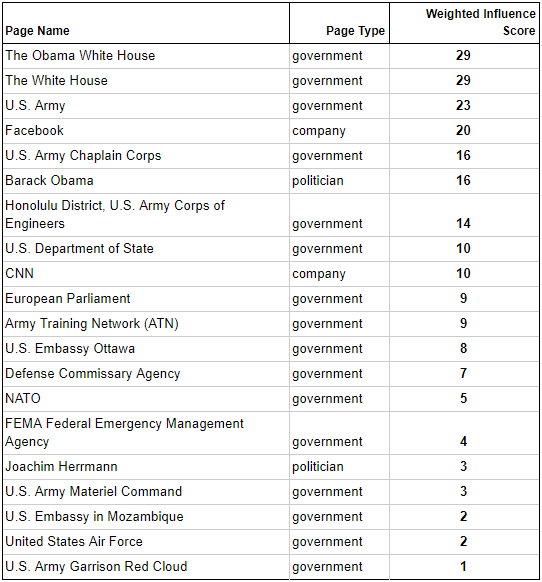
\includegraphics[scale=0.54]{weighted_influence_score.png} 
\caption{Weighted Influence}
\end{figure}


\section{Discussion}
This study attempts to derive and understand how to determine influence in a social media network. The research found that several nodes were high scoring in terms of both connectivity to other nodes: degree centrality, but also in most of the algorithmic centrality methods. In particular: “The Obama White House”,  “The White House”, “U.S. Army”, and “Facebook” appear to be highly influential in our network.  Further study could be done to discover how these nodes grew to be influential nodes overtime.  
 
The study looked closely at communities and found variability in community formation as defined by page type. The research found that government and company nodes were found in a large community but on the whole, the overall influential category of government nodes was found spread throughout various communities. A future study could look into how communities change over time with the emergence of new influential nodes. The node “The Obama White House” and “The White House” may be of particular interest because of the nature of the US presidency being of limited duration. A hypothesis would be that an updated dataset would find that the node “The Obama White House” would have reduced influences based on this study's metrics but of even more interest would be to see how the communities around these nodes evolved. 
 
More centrality methods and community detection algorithms and methods could be useful in the long term to derive an understanding of influence in the network. But the methods used in this study appear to be a good baseline. 
 
Besides, while this study focused on a social media dataset, the network science principles of centrality and communities could be applied to many other network types to identify how events or static ongoing influence impacts a network.  
 



\section{Conclusion}
Understanding influence in a network is important; groups spreading misinformation or the ability of a node to provide health information to the community at risk of a pandemic are several of many reasons among many to understand and utilize tools to identify and influence and communities in a social network. This study found that tools like Networkx package and Gephi are excellent tools to utilize to achieve the ends of this study as we seek a better understanding of social and other networks all around us.

\section{Acknowledgment}
Special thanks to professor Yong-Yeol Ahn and Jaehyuk Park for introducing multiple methods, concepts, and measurements in network science used in this paper.

\section{References}
\bibliography{references} 
\bibliographystyle{ieeetr}

\newpage

\appendixpage
\paragraph{Appendix A\newline\newline}
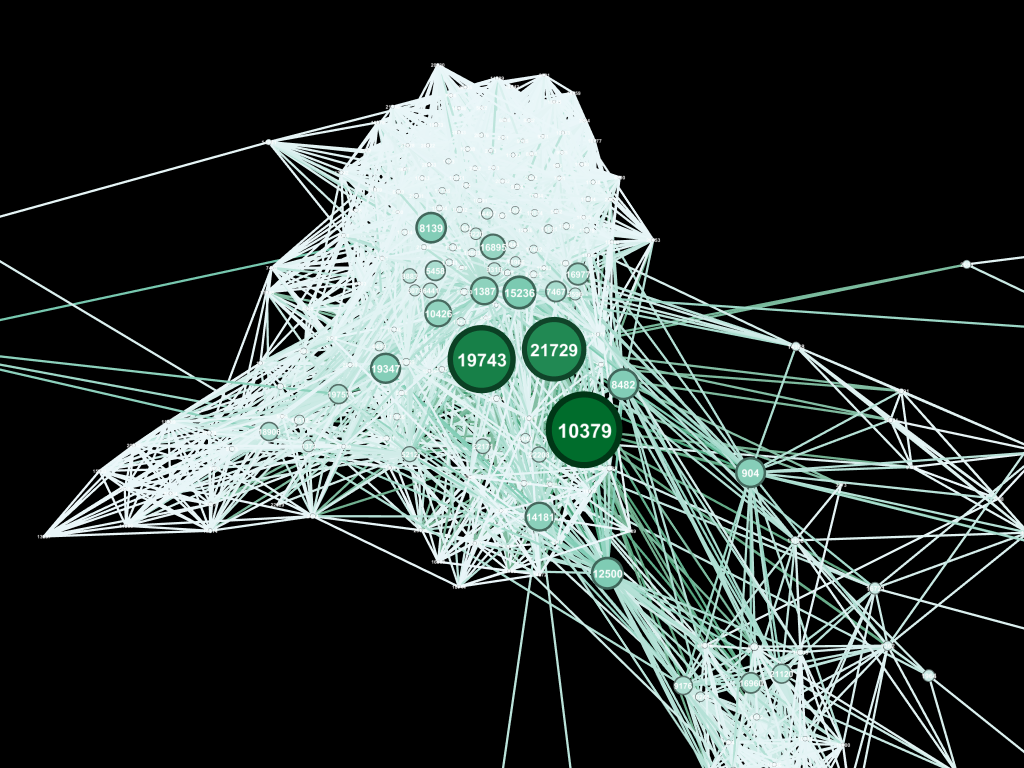
\includegraphics[scale=0.22]{betweennesscentraility_gov.png}
\paragraph{Appendix B\newline\newline}
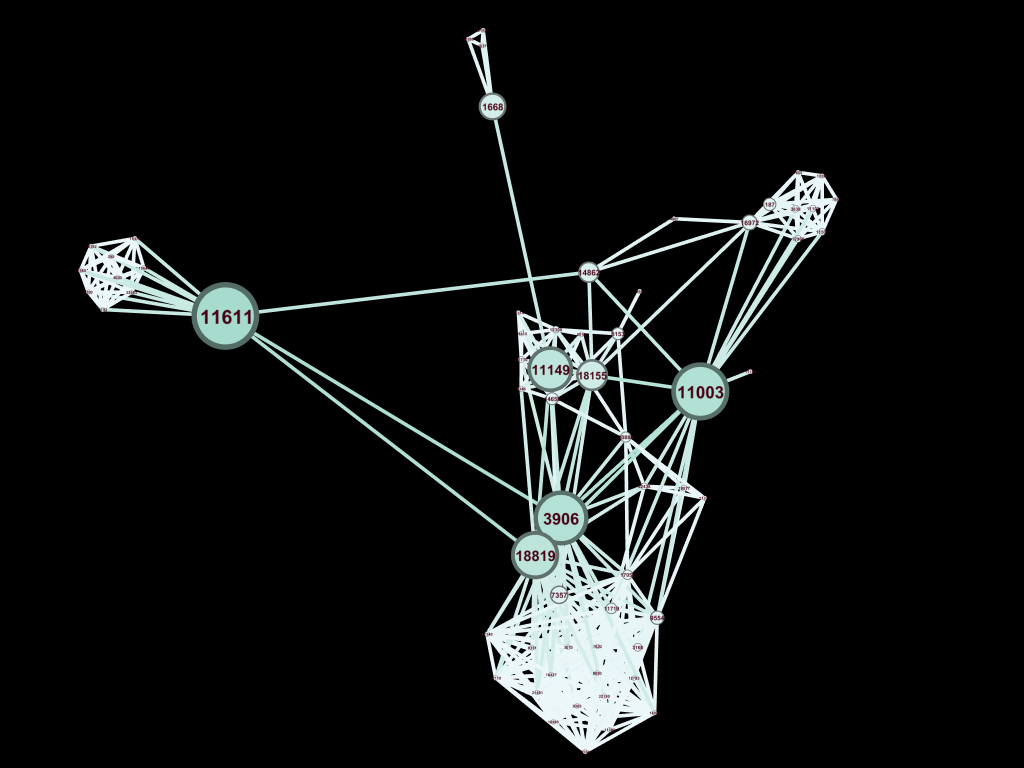
\includegraphics[scale=0.22]{betweennesscentraility_politician.png}
\newline
\paragraph{Appendix C\newline\newline\newline\newline\newline}
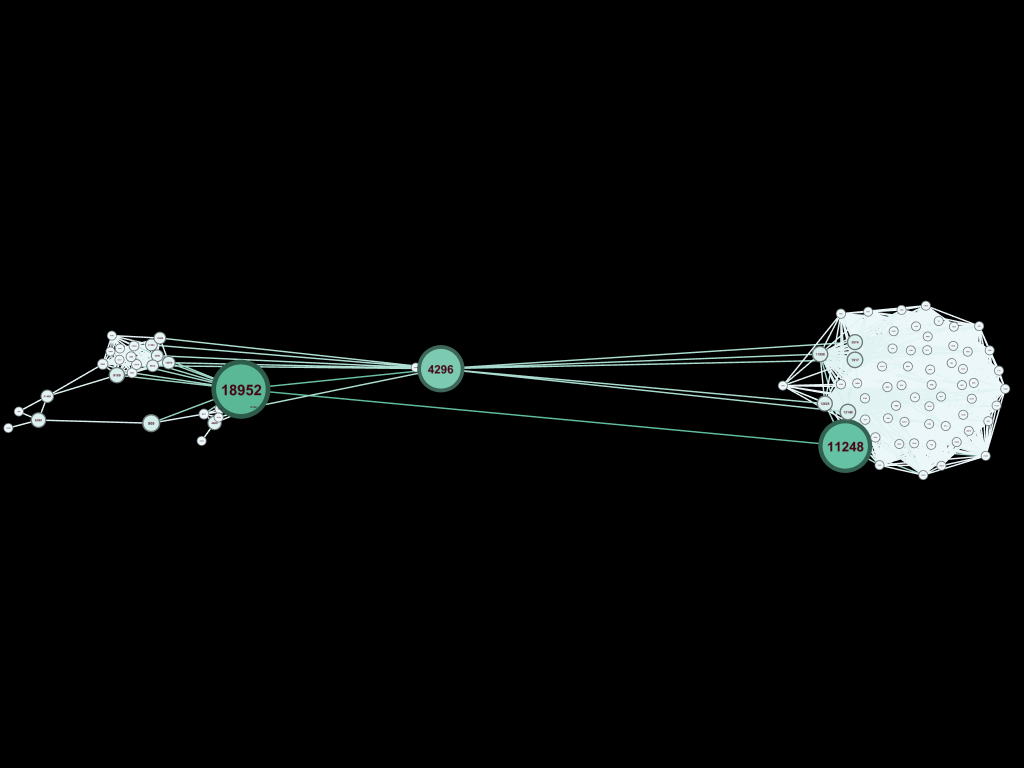
\includegraphics[scale=0.22]{betweennesscentraility_tvshow.png}
\paragraph{Appendix D\newline\newline\newline\newline\newline}
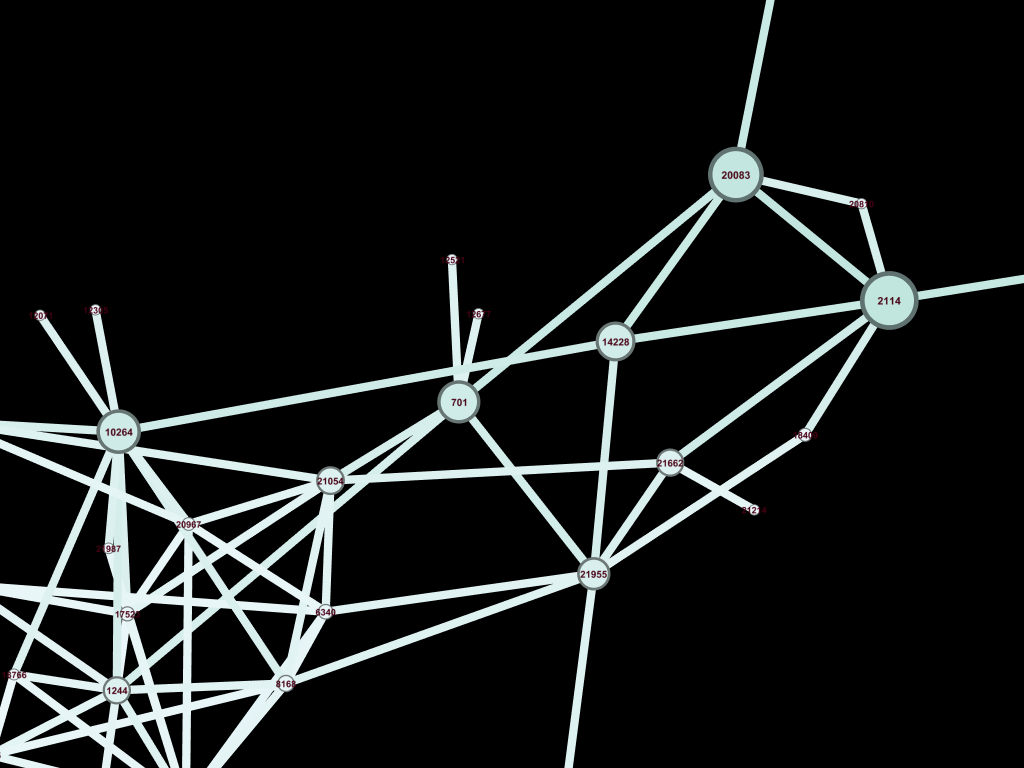
\includegraphics[scale=0.22]{betweennesscentraility_com.png}
\paragraph{{\newline\newline}Appendix E\newline\newline\newline\newline\newline}
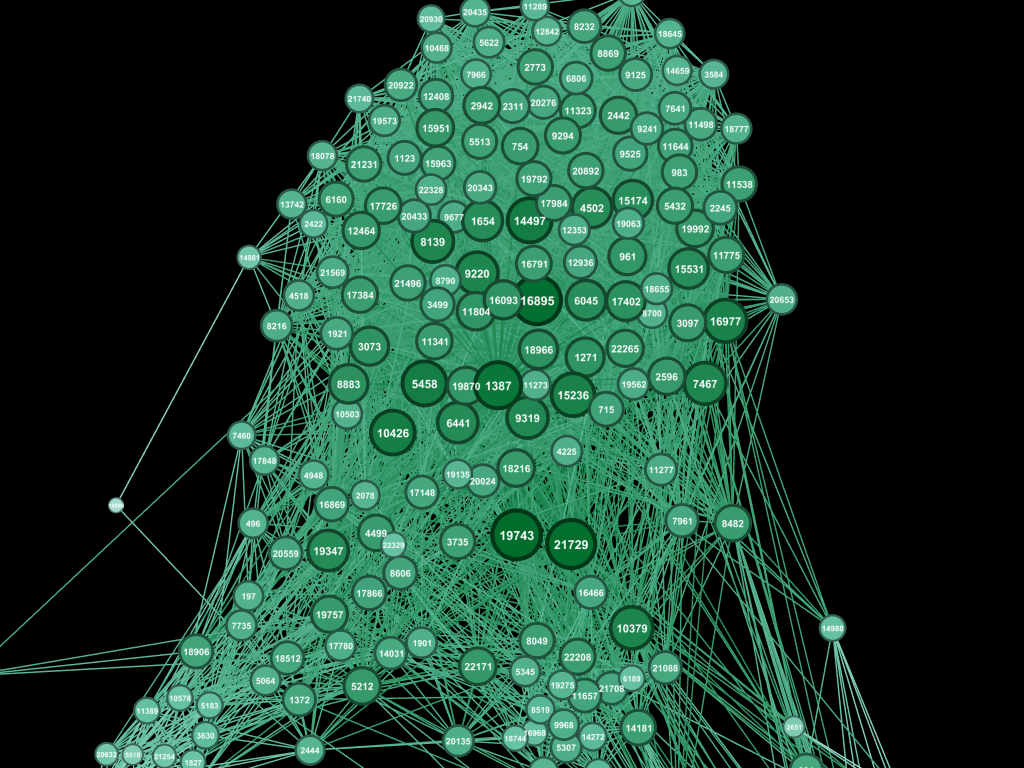
\includegraphics[scale=0.22]{closennesscentraility_gov.png}
\paragraph{{\newline}Appendix F\newline\newline\newline\newline\newline}
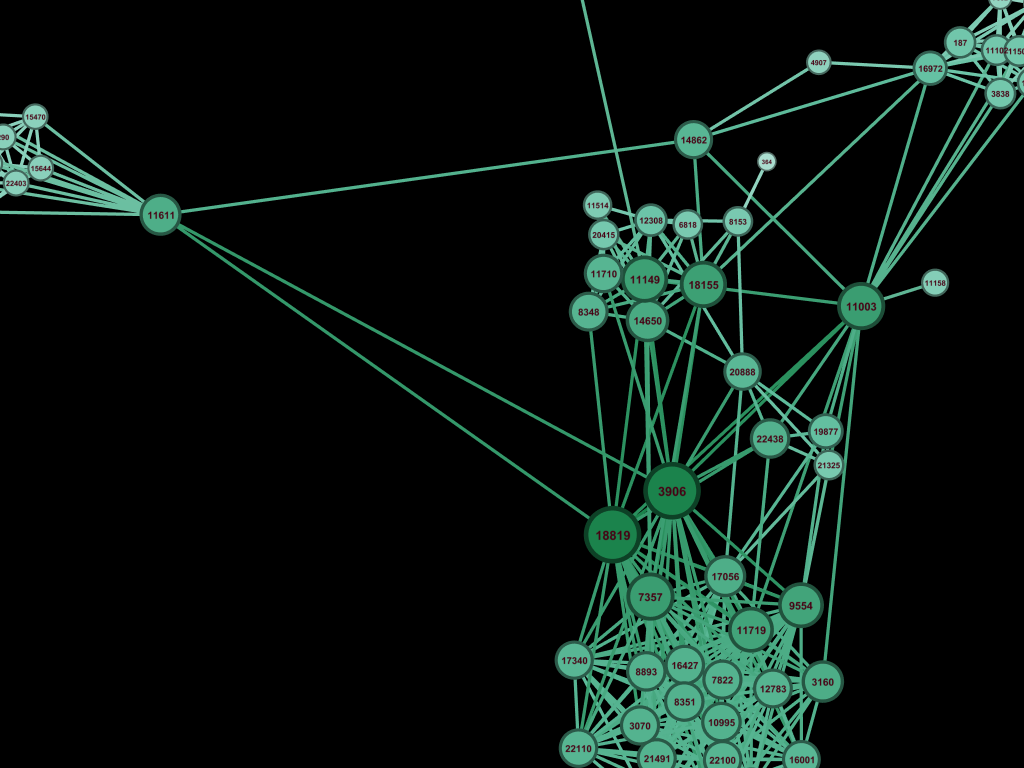
\includegraphics[scale=0.22]{closennesscentraility_pol.png}
\paragraph{Appendix G\newline\newline\newline\newline\newline}
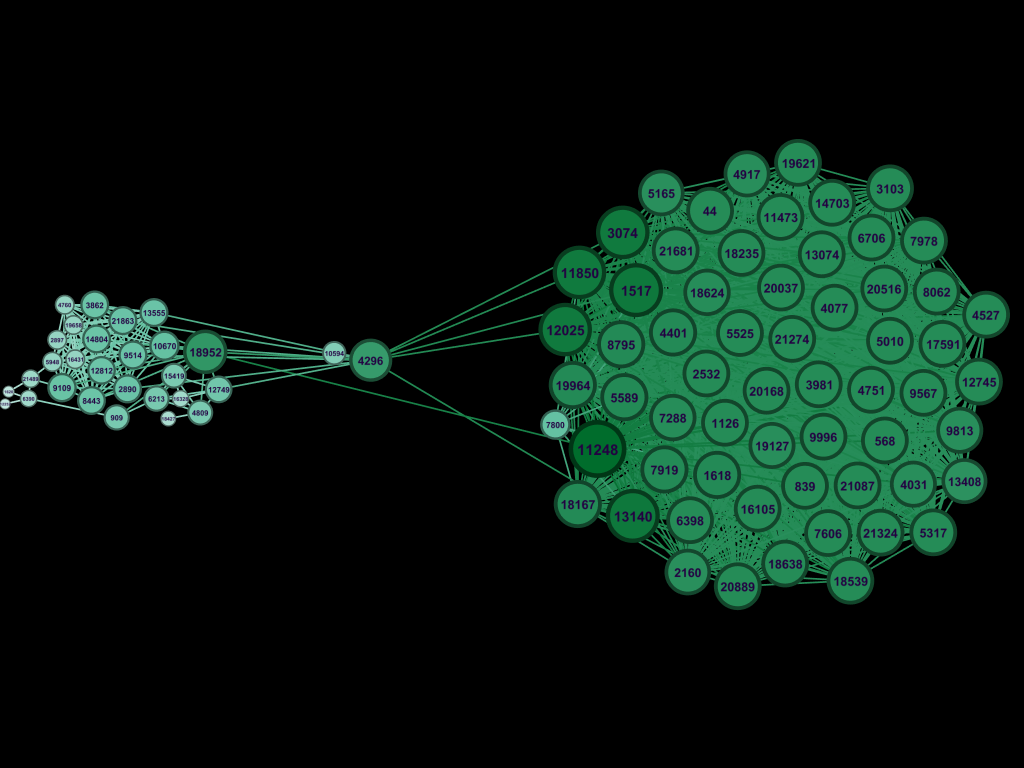
\includegraphics[scale=0.22]{closennesscentraility_tv.png}
\paragraph{{\newline}Appendix H\newline\newline\newline\newline\newline}
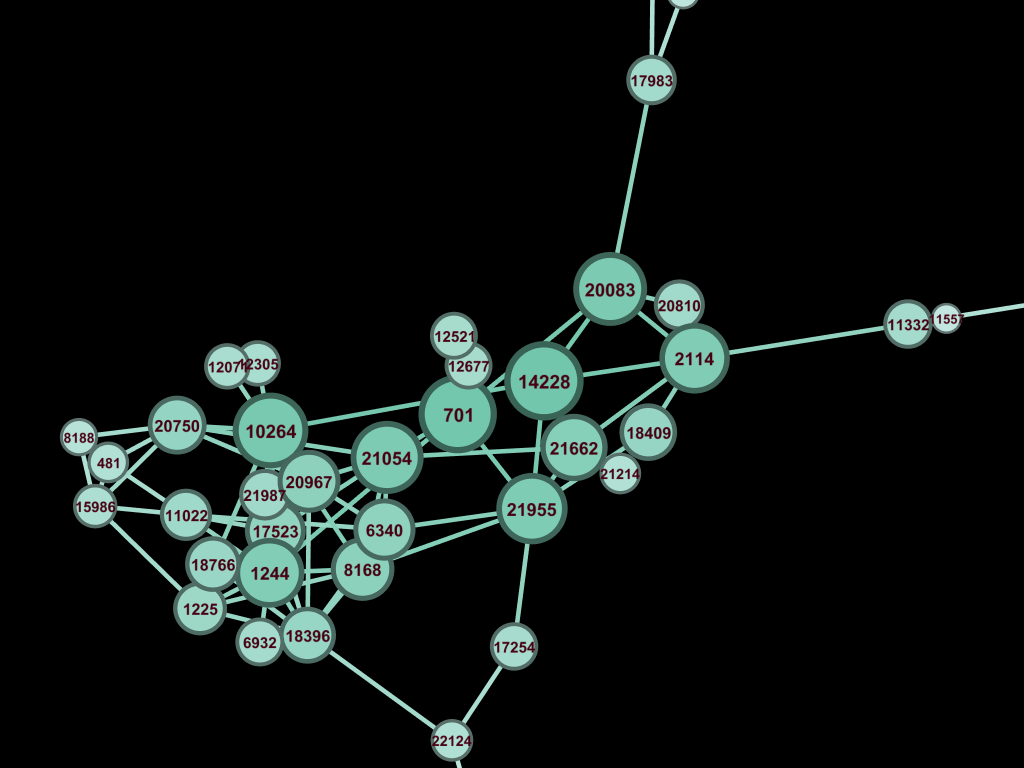
\includegraphics[scale=0.22]{closennesscentraility_com.png}
\paragraph{Appendix I\newline\newline\newline\newline\newline}
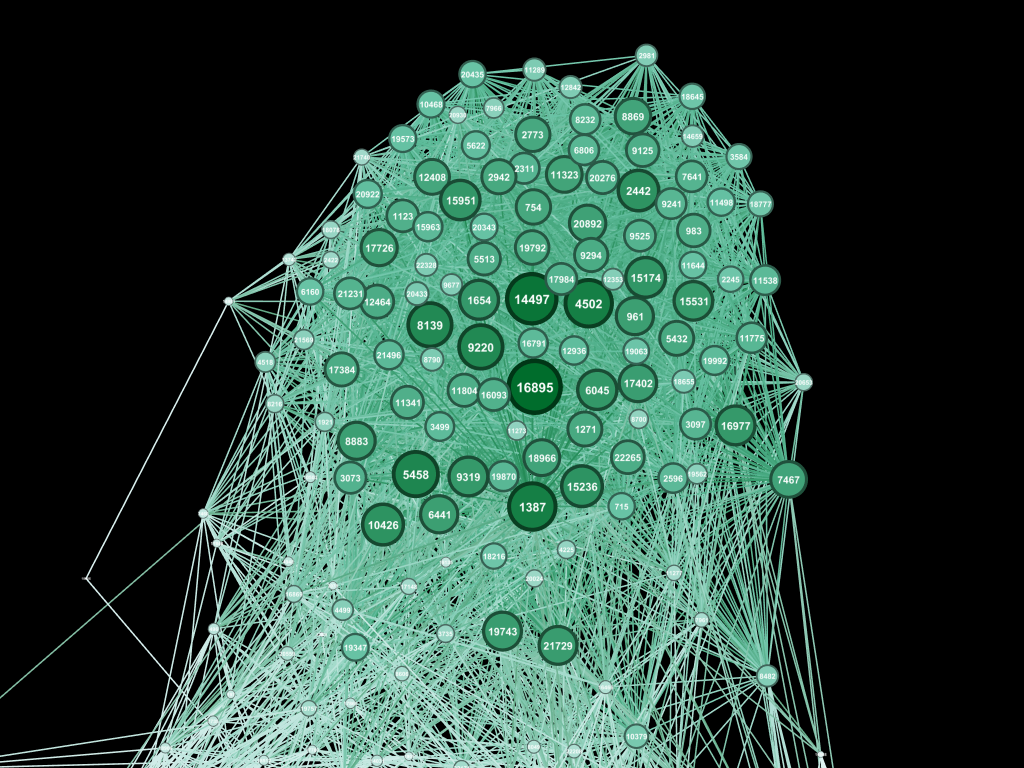
\includegraphics[scale=0.22]{eigenvectorcentraility_gov.png}
\paragraph{{\newline}Appendix J\newline\newline\newline\newline\newline}
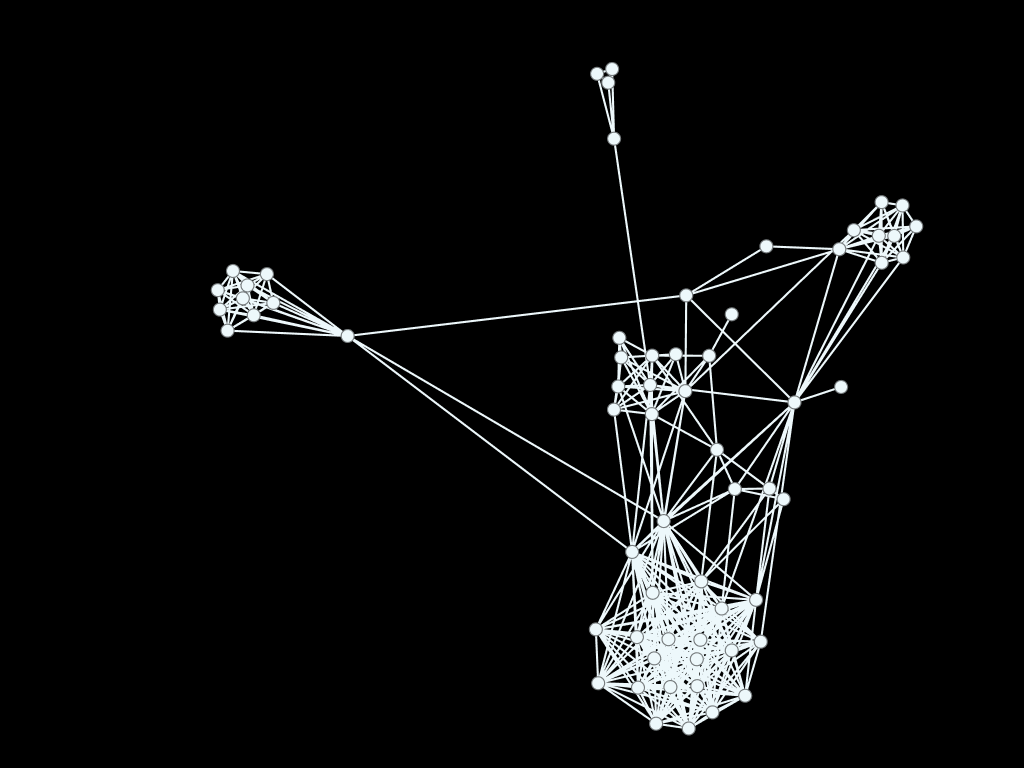
\includegraphics[scale=0.22]{eigenvectorcentraility_pol.png}
\paragraph{Appendix K\newline\newline\newline\newline\newline}
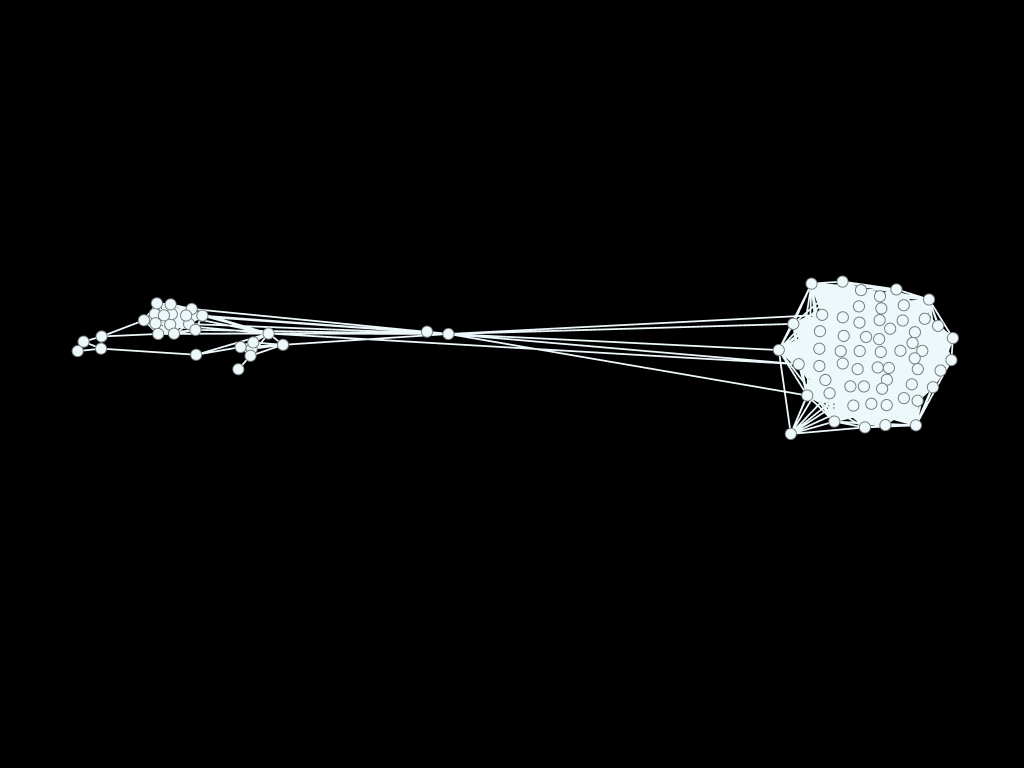
\includegraphics[scale=0.22]{eigenvectorcentraility_tv.png}
\paragraph{{\newline\newline\newline\newline}Appendix L\newline\newline\newline\newline\newline}
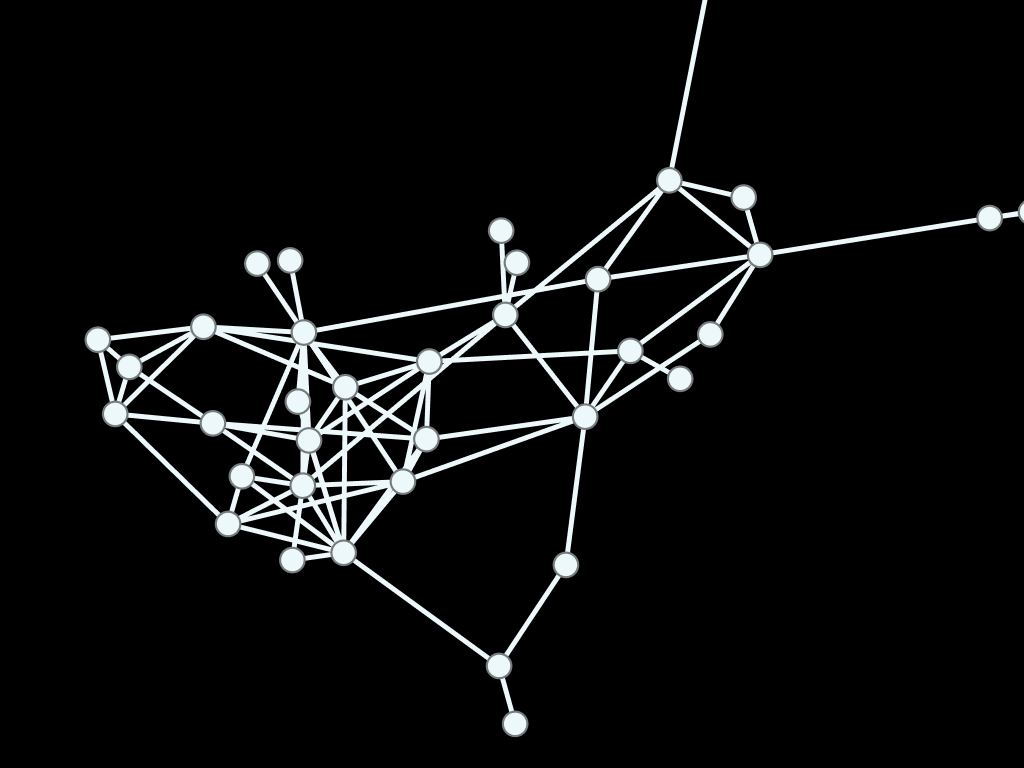
\includegraphics[scale=0.21]{eigenvectorcentraility_com.png}
\end{document}
